\documentclass[10pt]{beamer}

\usetheme{m}

\usepackage{booktabs}
\usepackage{graphicx}
\usepackage[scale=2]{ccicons}

\usepackage{pgfplots}
\usepgfplotslibrary{dateplot}

\title{Git Submodules}
\subtitle{An intro to managing dependencies}
\date{\today}
\author{Miguel Gonzalez and Jan Kerkenhoff}
\institute{Fontys Hogeschool Venlo}
% \titlegraphic{\hfill\includegraphics[height=1.5cm]{logo/logo}}

\begin{document}

\maketitle

\begin{frame}
  \frametitle{Table of Contents}
  \setbeamertemplate{section in toc}[sections numbered]
  \tableofcontents[hideallsubsections]
\end{frame}


\section{Introduction}

\begin{frame}
  \frametitle{Monoliths (really big projects!)}
  \begin{center}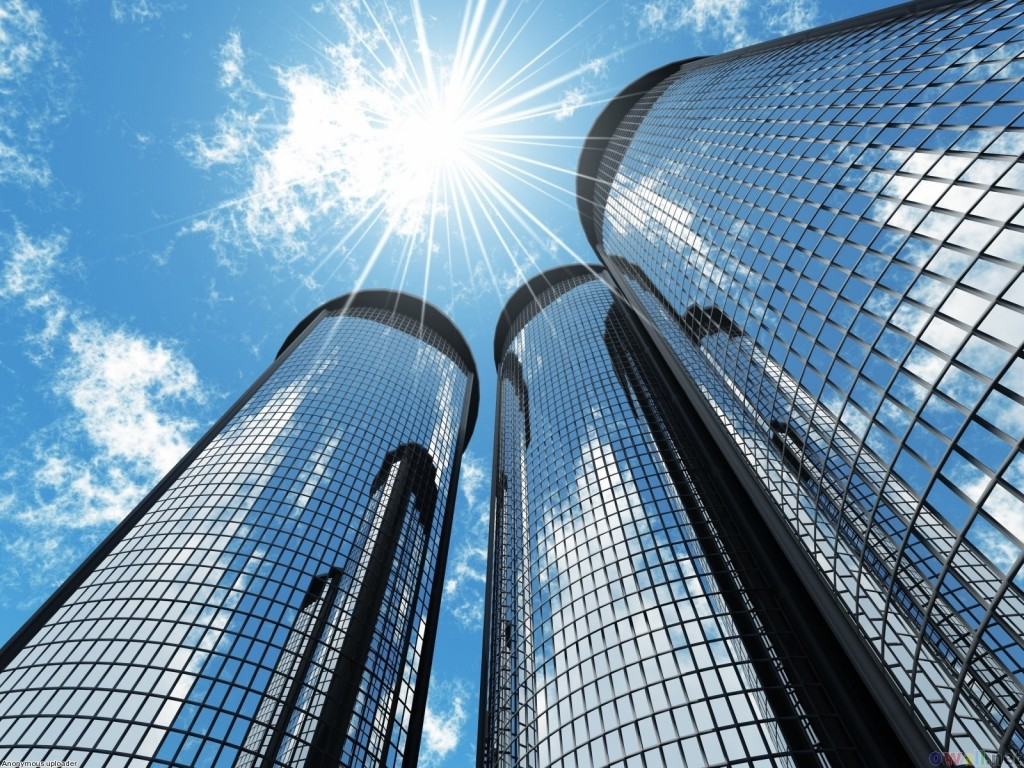
\includegraphics[width=280px]{images/monoliths.jpg}\end{center}
\end{frame}

\begin{frame}
  \frametitle{Monoliths (continued)}
  In terms of \textbf{git} there are a lot of drawbacks:
  \begin{itemize}
  	\item takes a long time to clone
  	\item many contributors
  	\item hard to keep track of all changes
  	\item wastes local disk space
  \end{itemize}  
\end{frame}

\begin{frame}
  \frametitle{the answer: git-submodules?}
  \begin{center}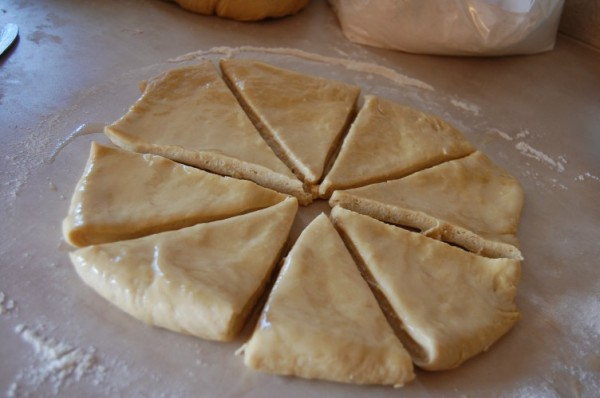
\includegraphics[width=280px]{images/divide.jpg}\end{center}
\end{frame}

\section{Pros and Cons}
\section{Live Demo}
\section{Updating Submodules}
\section{Working on Submodules}

\end{document}